\pagestyle{fancy}

\graphicspath{ {Figures/Chapter3_IntensitySimulation/} }

In this chapter, the signal generation in secondary emission monitors (SEM) when traversed by a particle beam will be covered. The formulations are going to be rather broad, for a generic particle beam and energy range. However, all the numerical examples will refer to SEM grids and Wire Scanner detectors in LINAC4. 

\section{Signal Generation in SEM}

At first, one can define the net charge generated on a wire or a foil transversed by a particle projectile (Proj) as: 

\begin{equation}
    \label{eq:Qsum}
    Q\left(\frac{e}{Proj}\right) = Q_{dep} + Q_{SE} + Q_{th}
\end{equation}

Where $Q_{dep}$ represents the charge generation due to Charge deposition. $Q_{SE}$ is the charge due to secondary emission and $Q_{th}$ is the charge due to thermionic emission. Figure \ref{fig:SignalGeneration} shows a schematic representation of the different processes that contribute to the charge generation in the material. They will be detaidely covered in the next sections. 

\begin{figure}[h]
    \centering
    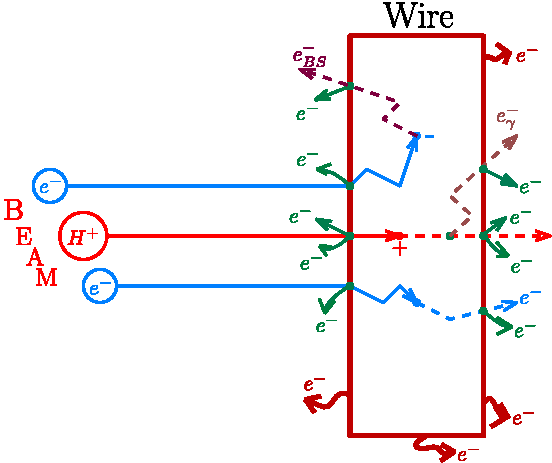
\includegraphics[width=0.50\columnwidth]{Figure_ChargeGeneration/ChargeGen.pdf}
    \caption{Schematic Representation of processes inducing current in the detector material.}
    \label{fig:SignalGeneration}
\end{figure}

\subsection{Charge Deposition ($Q_{dep}$)}

When an ion with $N_p$ number of protons in the nucleus and $N_e$ non-stripped electrons hits a target, the electrical charge directly deposited in the target depends on the probability of the protons and the electrons remaining on it. This can be written as: 

\begin{equation}
    Q_{dep} = N_p \cdot \eta - N_{e}\cdot \mu
\end{equation}

Where $\eta$ is the proportion of protons that are stopped in the material and $\mu$ is the proportion of electrons. These parameters depend on the range of the particles in the detector material, which was described in \ref{sec:Range}, and on the back-scattering probability, explained in \ref{sec:BS}. 

\subsection{Secondary Emission Charge ($Q_{SE}$)} 

The charge generated in the material by a particle, with $N_p$ number of protons and $N_e$ number of electrons, can be modeled as: 

\begin{equation}
    \begin{split}
        Q_{SE} = N_p \cdot SEY_{p1} + N_p \left(1-\eta\right)SEY_{p2} + 
                N_e \cdot SEY_{e1} + N_e \left( 1 - \mu \right) SEY_{e2} + \\
                N_p \cdot BS_p \cdot SEY_{BSp} + N_e \cdot BS_e \cdot SEY_{BSe}
    \end{split}
    \label{eq:Qse}
\end{equation}

Secondary emission is a surface process. In the case of a thin target detector, SE can occur at the entrance surface ($SEY_1$) and at the exiting one ($SEY_2$). And it can be induced by both the incident protons ($SEY_p$) and the electrons ($SEY_e$). In some cases, the probability of electron and proton backcattering ($BS_e$ and $BS_p$) is not negligible. In those cases, one must also consider the contribution of the secondary electrons generated due to the backscattered particles crossing twice the incident surface ($SEY_{BEp}$ and $SEY_{BEe}$).

In all the cases, SEY represents the secondary emission yield that was introduced in \ref{sec:SEY}. As was mentioned in the previous chapter, the semi empirical formula for secondary emission is valid at the entering surface as it does not account for energy loss in the material. For this reason in equation \ref{eq:Qse}, we specified the entrance surface as 1 and the exit surface as 2. One could try to obtain a more accurate description of the SE at the exit surface by accounting for the energy loss in the material. 

Similarly occurs with the back-scattering case. Backscattered particles might have different incident and exiting energies. If so,  $SEY_{BS}$ can be calculated more accurately. However, properly calculating the energy deposition induces some complications that, in some cases, might not be rewarded with a tangible improvement. 

\subsection{Thermionic Emissioon Charge ($Q_{Th}$)}
\label{sec:ThermoCurrent}
Thermionic emission is the process by which free electrons are emitted from the surface of a metal when they gain enough thermal energy to overcome the work function. As thermionic electrons are negative charges exiting the material surface, they will contribute to signal generation. $J_{Th}$ is the current density of emitted electrons and it is described by Richardson-Duschman equation \parencite[][]{ref:Richardson}:

\begin{equation}
    J_{Th} = A_R \cdot T^2 \cdot exp\left(-\frac{\phi}{k_B T} \right) 
    \label{eq:ThermoCurrent}
\end{equation}

$A_R$ is the Richardson constant and $K_B$ is Boltzmann's constant. From this equation, one can observe how dependent thermionic emission is on temperature. It is not until high temperatures are reached that thermionic emission can be detected. More on this will be explained in the following chapters. 

\section{LINAC4 Signal Generation Studies.}

As was introduced in \ref{sec:LINAC4}, LINAC4 accelerates \hm particles up to 160 MeV. \hm ions consist of one proton ($N_p$ = 1) and two electrons ($N_e$ = 2). In this case formula \ref{eq:Qsum} can be written as: 

\begin{equation}
    Q\left(\frac{e}{H^{-}}\right) = \eta - 2\mu + \left( 2 - \eta + BS_p \right) \cdot SEY_p +2\left( 2 - \mu - BS_e \right) \cdot SEY_e
    \label{eq:Ql4}
\end{equation}

Note that in this case, we are considering the secondary emission yield for electrons and protons to be the same at the entrance and the exit of the detectors. As we will see in the following, this might not be the most accurate procedure for some of the detectors at LINAC4. Figure \ref{fig:RangeLinac4} shows how the values of the range of protons change as a function of the particle energy. 

\begin{figure}[h]
    \centering
    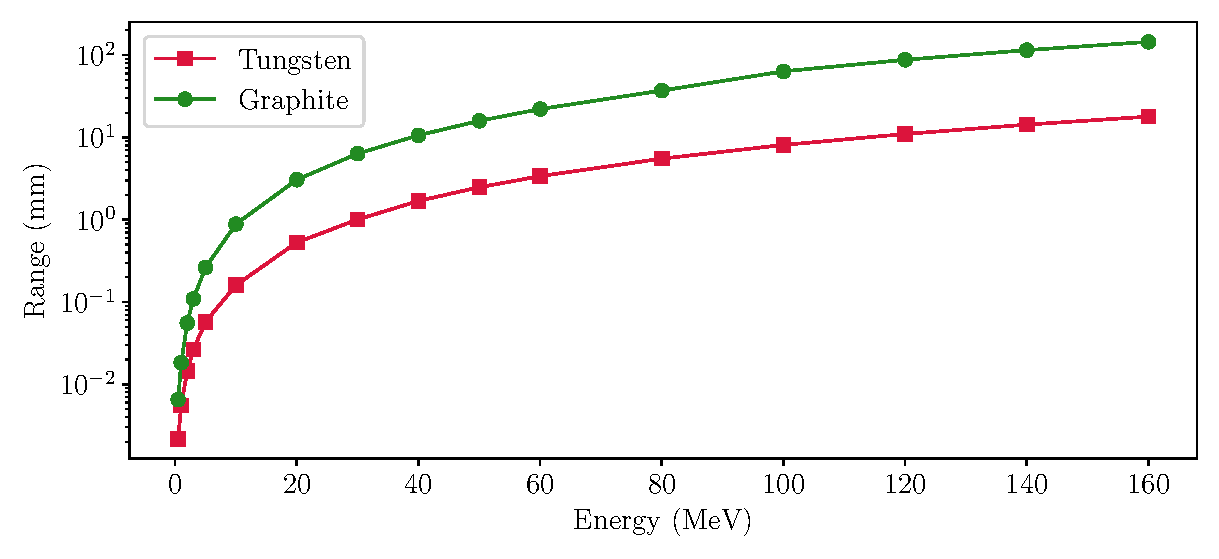
\includegraphics[width=0.9\columnwidth]{RangePlotLinac4/RangeL4.pdf}
    \caption{Range of particles as a function of incident ion energy.}
    \label{fig:RangeLinac4}
\end{figure}

From this figure, we can see how the range of the particles in the material increases as their energy increases. For the same energies, the particles have a much larger range in the case of graphite compared to tungsten. At LINAC4, the wires have a width of $40$ \si{\micro\metre} for the case of tungsten and 33 \si{\micro \metre} for the case of graphite wires. 

The range of protons is larger than the detector thickness in most of the energy range. Only tungsten detectors placed at energies smaller than 5  \si[]{\mega\electronvolt} are expected to get a positive charge deposition. The electrons in an \hm ion have energy much smaller than the proton. It is actually reduced a factor $m_p / m_e = 1836.15$ compared to the energy of the \hm ions.  Electrons are expected to deposit all their energy in all the SEM grids and Wire scanners at Linac4. So we expect to always have a double negative charge contribution. 

Table \ref{tab:ChargePar} summarizes the values for $\eta$ and $\mu$ parameters along the Linac4 accelerator range. This table also summarizes the values of the Backscattering probabilities for both electrons and protons. All these values have been calculated with Geant4 \parencite[][]{ref:Geant4}. The backscattering probability is negligible for the protons. Contrarily, electron backscattering probability is not negligible. In the case of tungsten, for ion energies of 160 MeV half of the electrons are backscattered.

% Please add the following required packages to your document preamble:
% \usepackage{multirow}
\begin{table}[h]
    \begin{tabular}{cccccccccc}
    \hline
    \multirow{2}{*}{\begin{tabular}[c]{@{}c@{}}$p^+$ energy \\ (MeV)\end{tabular}} & \multirow{2}{*}{\begin{tabular}[c]{@{}c@{}}$e^-$ energy\\ (keV)\end{tabular}} & \multicolumn{4}{c}{Graphite} & \multicolumn{4}{c}{Tungsten} \\ \cline{3-10}  &   & $\eta$   & $\mu$     & $BS_p$ & $BS_e$   & $\eta$ & $\mu$     & $BS_p$ & $BS_e$     \\ \hline
    3                                                                     & 1.63                                                                           & 0.001 & 0.918 & 0.0 & 0.081 & 1.0 & 0.632  & 0.0 & 0.367   \\
    50                                                                    & 27.23                                                                          & 0.0   & 0.931  & 0.0 & 0.068 & 0.0 & 0.506  & 0.0 & 0.493  \\
    102                                                                   & 55.55                                                                          & 0.0   & 0.887  & 0.0 & 0.112 & 0.0 & 0.487 & 0.0 & 0.512 \\
    160                                                                   & 87.14                                                                          & 0.0   & 0.857  & 0.0 & 0.142 & 0.0 & 0.464  & 0.0 & 0.536   \\ \hline
    \end{tabular}
    
    \caption{Summary of charge deposition and backscattering probabilities for Tungsten ($40 \mu m$) and Graphite ($33 \mu m$)} detectors.
    \label{tab:ChargePar}
\end{table}

Figure \ref{fig:SEYmat} shows the Secondary Emission yield calculated with the semiempirical Sternglass formula (Eq. \ref{eq:sey}) as a function of the incident proton energy.  In both materials, the SEY reaches a maximum ( $~ 0.1 $ MeV ) which is followed by a decrease in the SEY. Graphite presents a higher SEY at smaller proton energies whereas tungsten presents a higher SEY at higher incident particle eneriges. 

\begin{figure}[h]
    \centering
    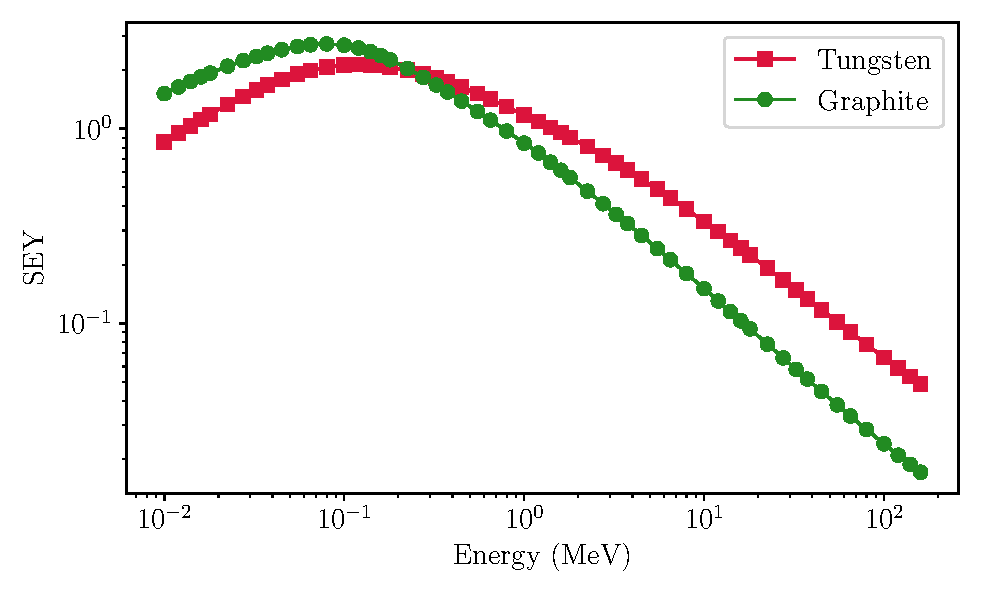
\includegraphics[width=0.85\columnwidth]{Figure_SEY/SEY_compa.pdf}
    \caption{Secondary Emission Yield as a function of incident proton energy. }
    \label{fig:SEYmat}
\end{figure}

As an example, figure \ref{fig:ProfComparison} shows a simulated beam profile at 3 MeV and 160 MeV. From these figures, we can observe how at 3 (MeV) the positive contribution to the charge is predominant for the case of tungsten wires while it remains negative in the case of graphite wires. Due to the smaller SEY of graphite at 160 (MeV), the absolute registered signal at this energy is higher than the one registered by the tungsten wires. 

\begin{figure}[h]
    \centering
    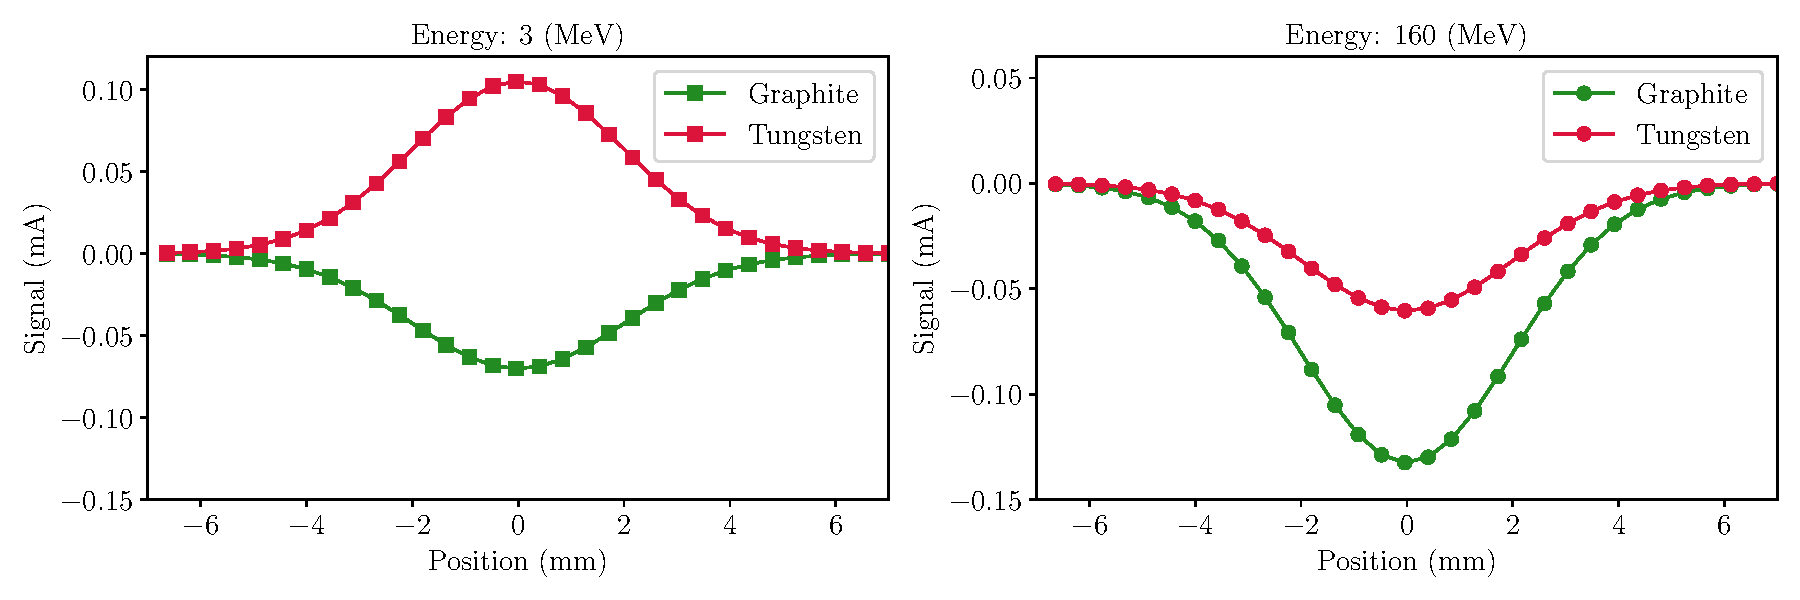
\includegraphics[width=0.85\columnwidth]{Figure_ProfCompa/ProfileComparison.pdf}
    \caption{Expected transverse beam profile for incident \hm particles. Left: 3 (MeV), Right: 160 (MeV). For these simulations, a 25 mA, 100 $\mu s$ particle beam was considered. }
    \label{fig:ProfComparison}
\end{figure}

At Linac4, even if these detectors are called Secondary Emission Monitors, the biggest contribution to the charge formation is the charge deposition term. To prevent misinterpretations, SE is typically suppressed by a bias current.  At LINAC4, the detectors at lower energies are usually conformed with graphite wires, to avoid the positive contribution of the proton charge deposition. 

\section{Beam Intensity and Profile Measurements at CERN LINAC4.}

In this section, we will briefly show how the instruments just presented are used at CERN, LINAC4. All the results presented in this section correspond to the first profile and current measurements for the LBE run, which took place in November 2019 \parencite*[][]{ref:PresentationLBERun}. The objective of these measurements was to study the transverse profile evolution of the particle beam along the LINAC4 accelerator. 

Figure \ref{fig:Linac4Layout} shows a schematic representation of LINAC4 with the different detectors and locations. In this figure, the yellow circles represent the BCTs. The blue and red rectangles indicate the positions of SEM grids and Wire scanners respectively. Green rectangles indicate positions where SEM grid and Wire scanners are installed at the same position. As we can see from this figure, both BCTs and Beam profile instruments are placed all along LINAC4 so the beam parameters can be measured in all the acceleration stages. 

\begin{figure}[h]
    \centering
    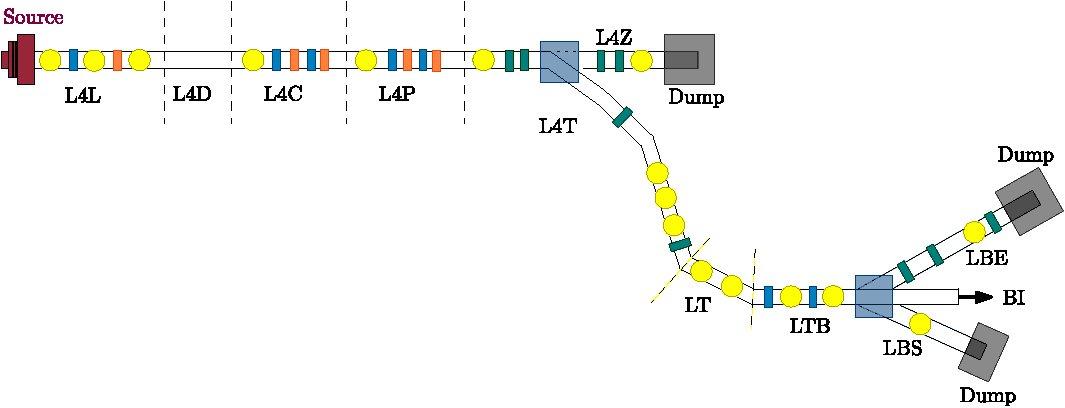
\includegraphics[width=1.0\columnwidth]{Linac4Instrumetnation/Linac4Instruments.pdf}
    \caption{Schematic representation of LINAC4 with the location of some diagnostics devices.}
    \label{fig:Linac4Layout}
\end{figure}

Figure \ref{fig:BCTwithTime} shows an example of intensity measurement taken by the first BCT in the L4T segment. From this figure, one can identify the beam pulse, we can observe that due to the accelerator of $H^{-}$ particles at LINAC4, the registered current is negative. In this case, the beam pulse length was 36 \si[]{\micro \second} with an average intensity of $\sim 17 $ \si[]{\milli \ampere}. One can observe the 1 \si[]{\micro \second} gaps generated by the chopper, which make the beam pulse ready to be injected into the different pulse rings. 

\begin{figure}
    \centering
    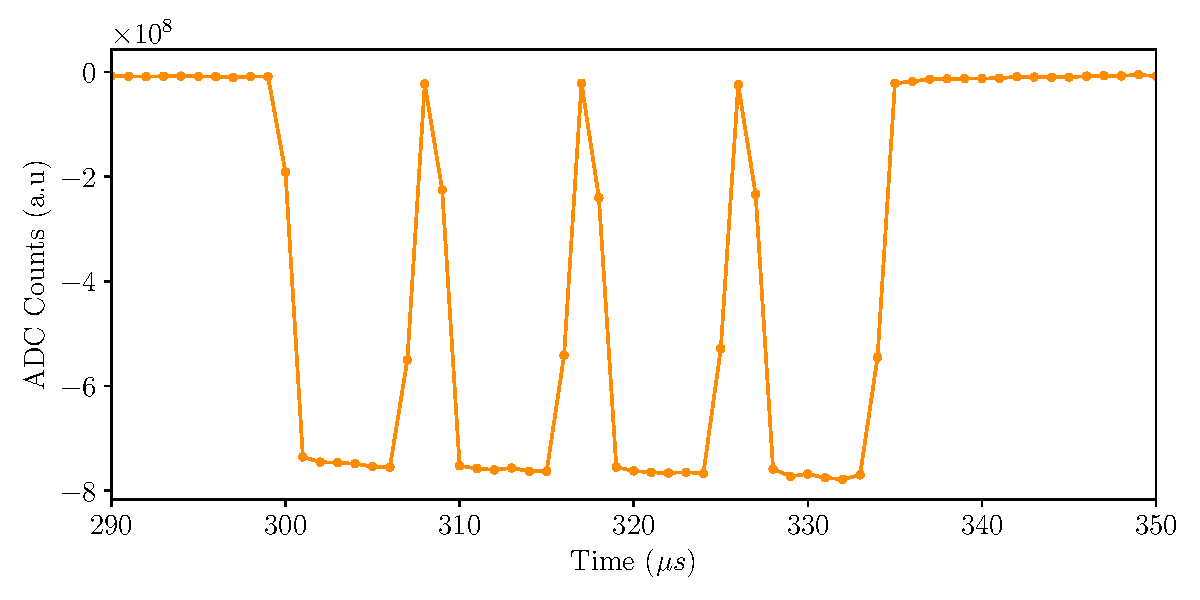
\includegraphics[width=0.7\columnwidth]{IntensityVStime/IntensityVStime.pdf}
    \caption[The LOF caption]{Beam current shape along beam pulse, from first BCT in L4T line.}
    \label{fig:BCTwithTime}
\end{figure}

By measuring the average current of the beam at all the available BCTs, one can assess the beam transmission along the accelerator. Figure \ref{fig:BeamTrans} shows an example of beam transmission measured along the accelerator. From this figure one can observe how in all parts of the accelerator, except for the first two BCTs in the L4L line, the current remains quite constant around $\sim 17$ \si[]{\milli \ampere}.  Similarly, the beam transmission remains very close to $100 \%$ along the whole accelerator. 

\begin{figure}
    \centering
    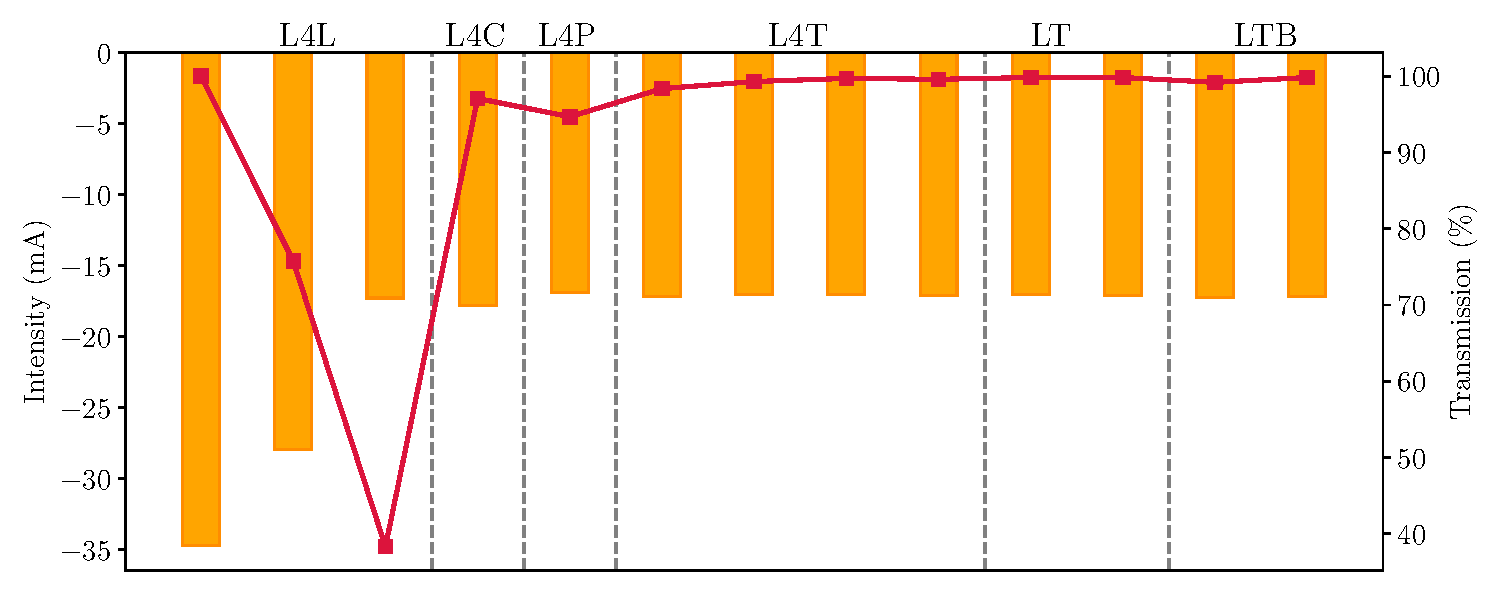
\includegraphics[width=0.9\columnwidth]{BCT_Transmission/TransmissionBCT.pdf}
    \caption{Average intensity measured by the different BCTs at LINAC4. Transmission along the LBE line.}
    \label{fig:BeamTrans}
\end{figure}


Similarly, the beam profile was measured along the accelerator, to cross-check the beam evolution as well as to assess the integrity and status of the devices installed along the accelerator.  Figure \ref{fig:HorizontalProf} shows the measurements of the horizontal profile of the beam along the LINAC4 accelerator. All these measurements were taken with the SEM grids. From this figure we can observe:

\begin{figure}
    \centering
    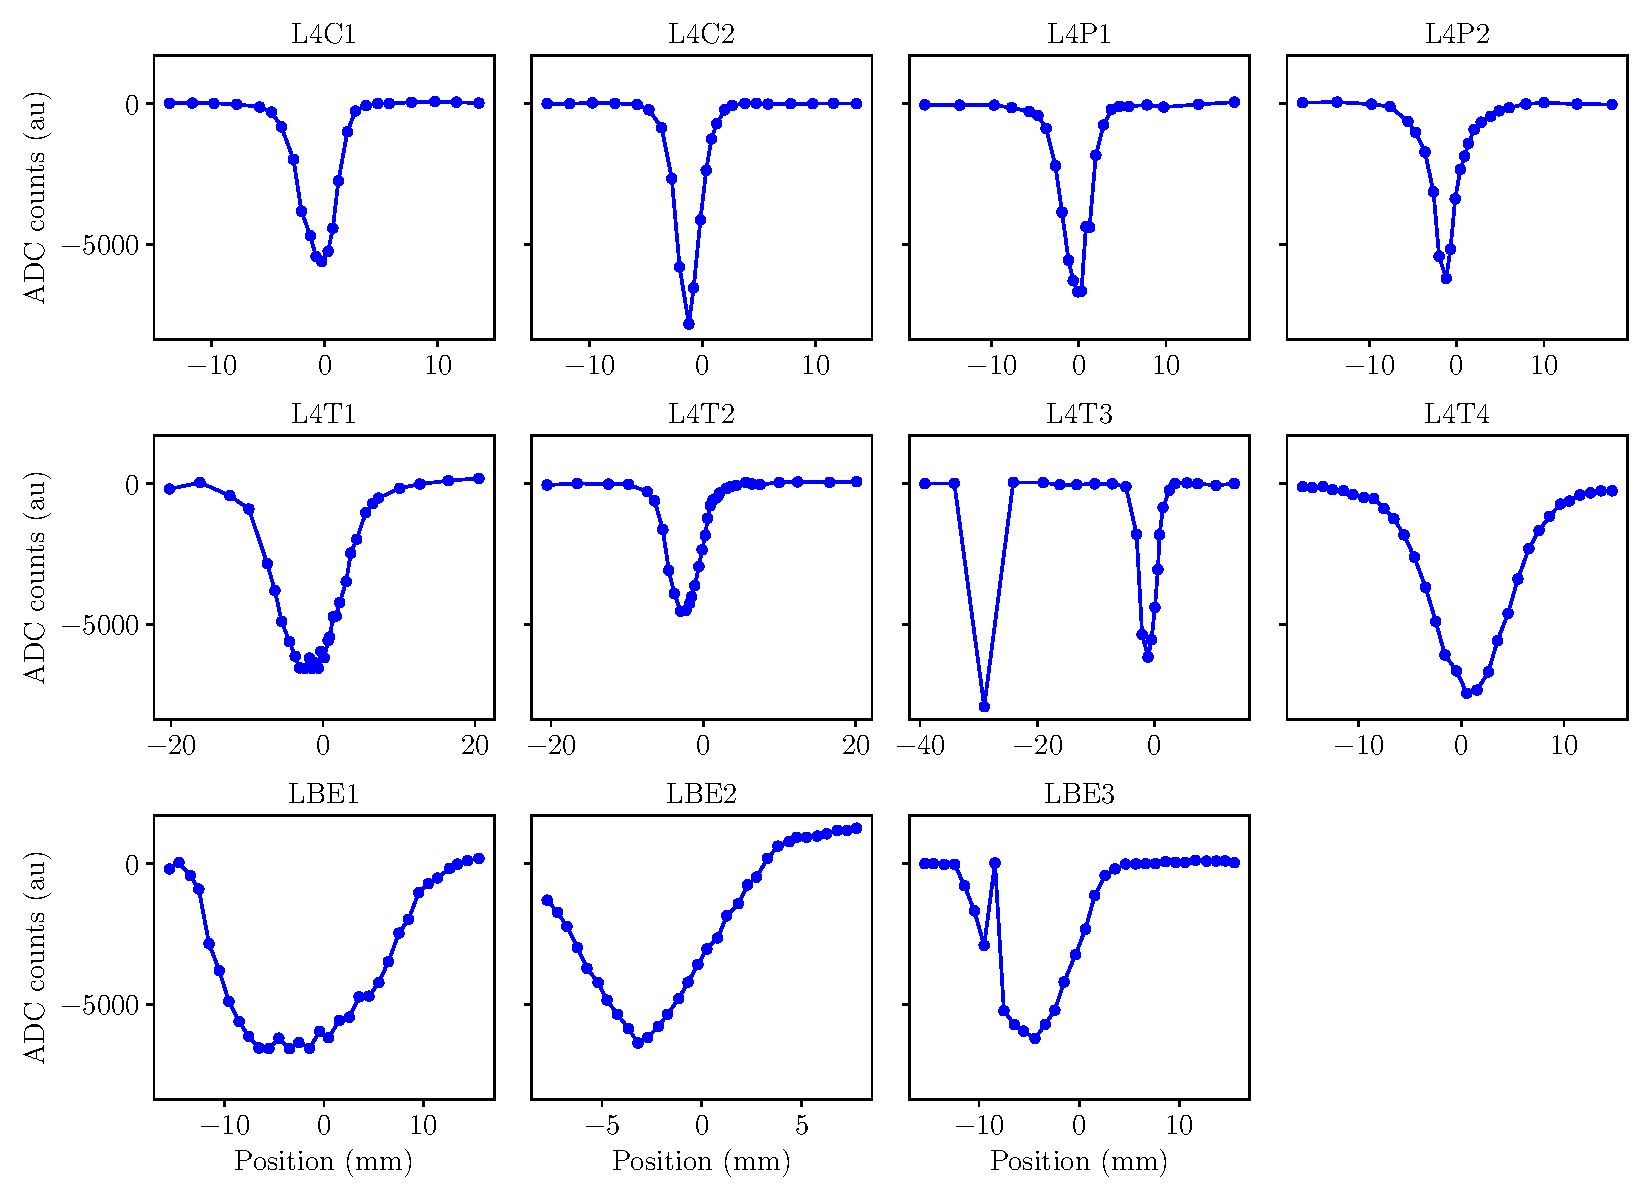
\includegraphics[width=1.0\columnwidth]{SigmaEvol/HorEvol.pdf}
    \caption{Horizontal transversal beam profile measured by the differt detectors at LINAC4}
    \label{fig:HorizontalProf}
\end{figure}

\begin{itemize}
    \item The beam profile seemed to be very much gaussian in all the measurement points except for LBE1 and LBE2 positions.
    \item Broken wires: SEM grids L4T2 and LBE3 present a broken wire that must be repaired. Wires 12-13 and 14-15 in L4P1 are glued together. 
    \item L4T1 and LBE1 present strange strange oscillations in the wires measuring the highest intensities. 
    \item Some of the grids have an even wire separation while others present a noneven wire distancing. Due to the beam not always being centered having smaller wire separation at the center of the grid des not seem to be that helpful.
    \item Not depicted, however, the data acquisition system for the detectors in the LBE sector had to be corrected to properly acquire the data.
\end{itemize}

Here we presented only the evolution of the horizontal profile, however, the evolution of the vertical profile was similarly studied. In the case of the vertical profile, a non-gaussian beam was observed in some of the locations. Figure \ref{fig:VertProf} shows an example of a vertical profile taken with both the second SEM grid and the second Wire Scanner from the L4T line. In this case, the particle beam clearly shows some shoulders or tails that push it away from the gaussian distribution. Another thing that one can observe from this figure, is the great agreement between the beam profile measurements by the sem grid and the wire scanner. 


These measurements were the first systematic set of measurements of the LBE run, they helped understand the beam evolution along the accelerator and thus helped correct the observed irregularities. These measurements also helped assess and correct any issue on the measuring devices, such as broken wires, position misreadings, data acquisition problems, etc.  

\begin{figure}[h]
    \centering
    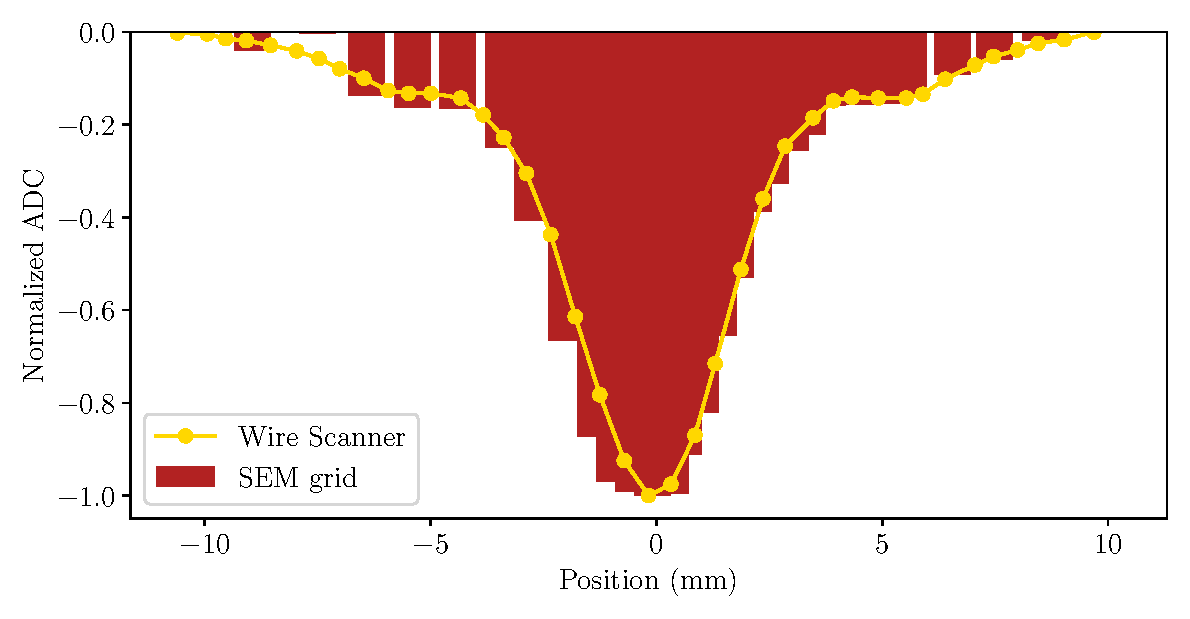
\includegraphics[width=0.6\columnwidth]{VertProf/VertProf.pdf}
    \caption{Vertical transverse profile measured by the second SEM grid and second wire scanner of the L4T line at Linac4.}
    \label{fig:VertProf}
\end{figure}




